\subsection*{Дискретные СВ и случайные события}
\addcontentsline{toc}{subsection}{Дискретные СВ и случайные события}

\textbf{Задание:}\\
Используя метод статистических испытаний, оценить вероятность выпадения герба при бросании правильной монеты. Проанализируйте, как зависит точность полученного результата от количества точек, использованных для получения оценки. Постройте график этой зависимости.\\

\textbf{Решение:}\\
Для решения данной задачи стоить сгенерировать $n$ случайных равномерно распределённых чисел, если $x_i < 0.5$, то добавлять в результирующий список 0, в противном случае 1. Далее стоит просуммировать элементы получившегося списка и разделить на количество элементов в этом списке.\\

Данный алгоритм был реализован на языке программирования Python. (Рисунок \ref{fig:coin_code})
\begin{figure}[h]
	\centering 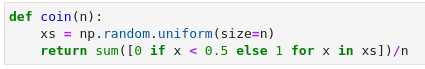
\includegraphics[scale=0.65]{coin_code}
	\caption{Реализация метода статистических испытаний}
	\label{fig:coin_code}
\end{figure}

Также была проанализирована зависимость между точностью результата и количеством сгенерированных точек. (Рисунок \ref{fig:coin_result})
\begin{figure}[h]
	\centering 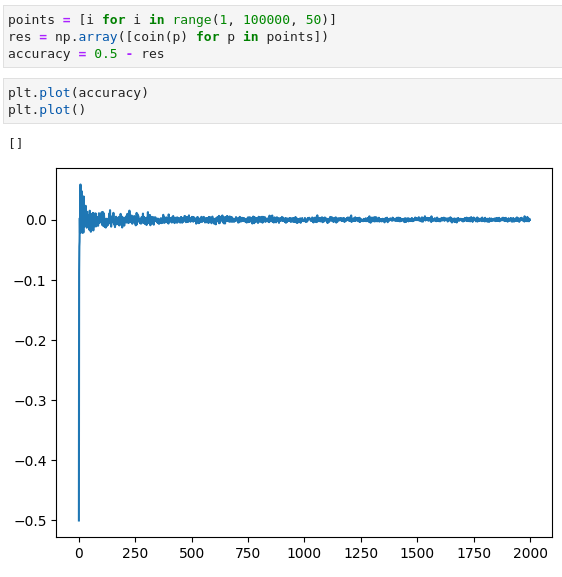
\includegraphics[scale=0.4]{coin_result}
	\caption{Зависимость точности результатов от количества точек}
	\label{fig:coin_result}
\end{figure}

Как можно видеть на графике, что чем больше количество сгенерированных точек, то тем точнее получается результат.